%%%%%%%%%%%%%%%%%%%%%%%%%%%%%%%%%%%%%%%%%%%%%%%%%%%%%%%%%%%%%%%%%%%%%%%%%%%%%%
%
% Section file included in main project file using \input{}
%
% Assumes that LaTeX2e macros and packages defined in cg_comp.sty are
%   available
%
%%%%%%%%%%%%%%%%%%%%%%%%%%%%%%%%%%%%%%%%%%%%%%%%%%%%%%%%%%%%%%%%%%%%%%%%%%%%%%

 \section{Classical Guitar Compensation\label{sct:comp}}

 In \sct{model}, we noted that the bending stiffness and the increase in string tension due to fretting sharpen the pitch, but that we can flatten it with a positive saddle setback and negative nut setback. In \app{rms}, we develop an RMS least-squares fit method that numerically solves \eqn{error_def} for the values of $\Delta S$ and $\Delta N$ that minimize the root-mean-square of the frequency errors of a string over a particular set of frets. In the case of our Classical Guitar with normal-tension nylon strings --- shown in \fig{shift_classicalguitar_ej45_null} for the case of zero setbacks --- we use this method with $d = 0$ to obtain the nonzero setbacks listed in \tbl{ej45_setbacks}. The corresponding frequency deviations are shown in \fig{shift_classicalguitar_ej45_full} (assuming that all other aspects of the guitar remain unchanged). Of course, manufacturing a guitar with unique saddle and nut setbacks for each string (of a particular tension) can be challenging, so we also plot in \fig{shift_classicalguitar_ej45_mean} the shifts obtained by setting each of the values of $\Delta S$ and $\Delta N$ to the mean of the corresponding column in  \tbl{ej45_setbacks}. In both cases, the RMS error is significantly smaller than that of the uncompensated guitar shown in \fig{shift_classicalguitar_ej45_null}.

 \begin{figure}
  \centering
  \begin{subfigure}[b]{0.8\textwidth}
   \centering
   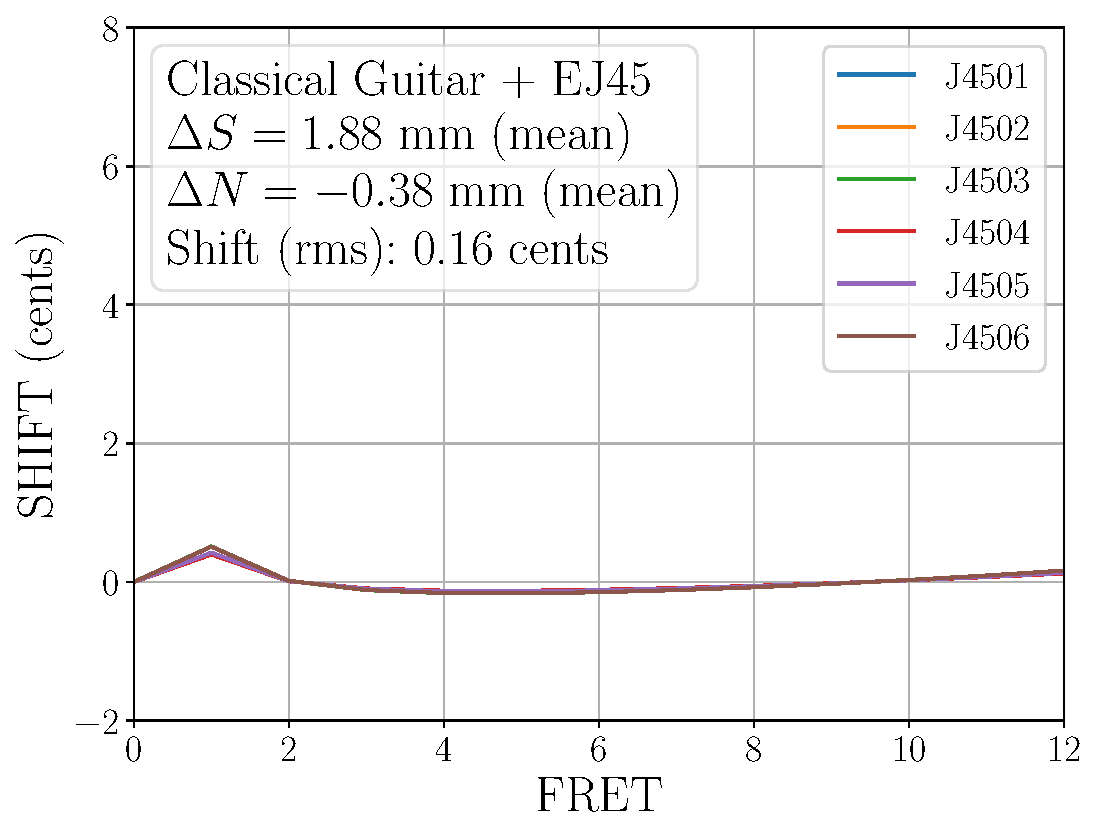
\includegraphics[width=5.0in]{figures/shift_classicalguitar_ej45_full}
   \caption{Full compensation}
   \label{fig:shift_classicalguitar_ej45_full}
  \end{subfigure}
  \par\vspace{0.25in}
  \begin{subfigure}[b]{0.8\textwidth}
   \centering
   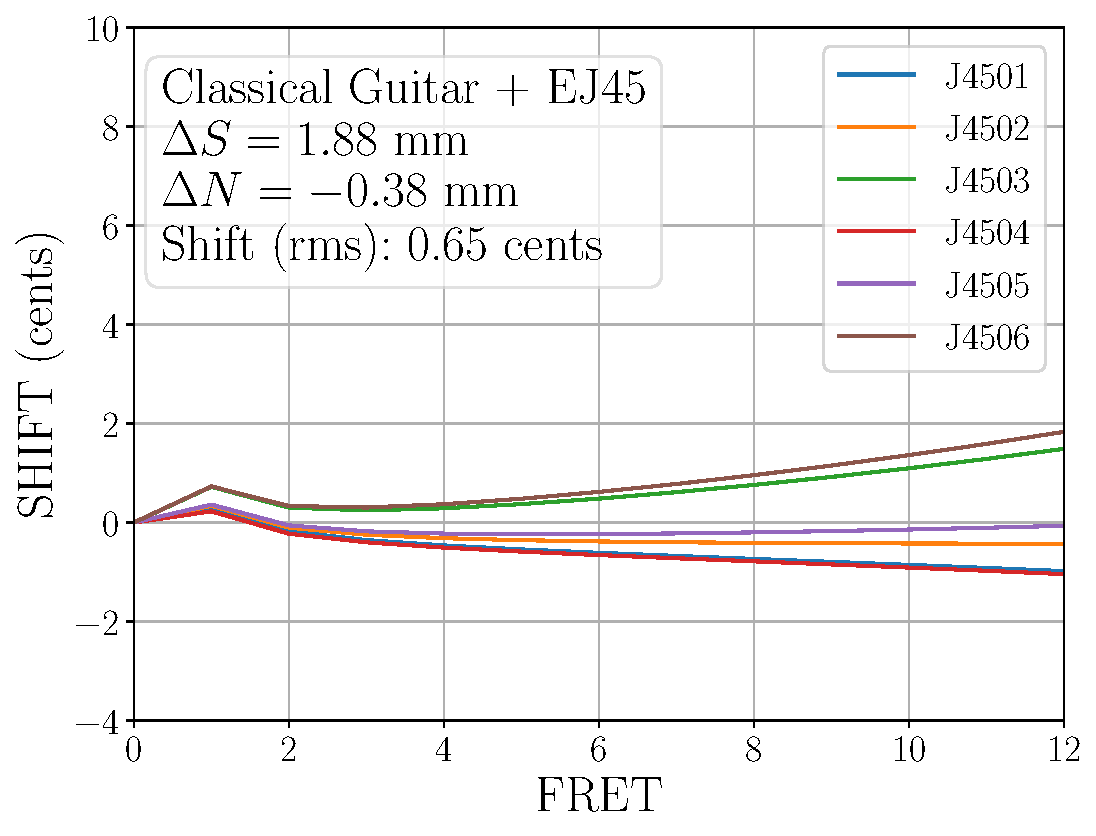
\includegraphics[width=5.0in]{figures/shift_classicalguitar_ej45_mean}
   \caption{Mean compensation}
   \label{fig:shift_classicalguitar_ej45_mean}
  \end{subfigure}
  \caption{\label{fig:compensation_classicalguitar_ej45} Frequency shifts (in cents) for the Classical Guitar with normal tension nylon strings (D'Addario EJ45). In (a) we use the individual values for each string that are listed in \tbl{ej45_setbacks}. In (b), we set $\Delta S$ and $\Delta N$ to the mean of the corresponding column in that table.}
 \end{figure}

 \begin{table}[htbp]
  \centering
  \caption{\label{tbl:ej45_setbacks} Predicted setbacks for the D'Addario Pro-Arte Nylon Classical Guitar Strings -- Normal Tension (EJ45) on the Classical Guitar.}
  \begin{tabular}{cccc}
\toprule
String &  $\Delta S$ (mm) &  $\Delta N$ (mm) &  $\overline{\Delta \nu}_\text{rms}$ (cents) \\
\midrule
 J4501 &             2.16 &            -0.43 &                                        0.18 \\
 J4502 &             1.92 &            -0.31 &                                        0.15 \\
 J4503 &             4.36 &            -0.82 &                                        0.31 \\
 J4504 &             1.30 &            -0.19 &                                        0.13 \\
 J4505 &             1.94 &            -0.28 &                                        0.15 \\
 J4506 &             2.62 &            -0.35 &                                        0.16 \\
\bottomrule
\end{tabular}


\end{table}%


% Note that the saddle setbacks tend to be larger --- and the nut setbacks smaller --- than the simple estimates that we made above for a hypothetical thick string. This is easily understood by examining \eqn{error_tot}: the portion of $\Delta S$ that exceeds $B_0\, X_0$ scales with $\gamma_n - 1$, and helps to compensate for tension errors as $n$ increases.
This purely numerical approach using \eqn{error_def} is accurate but not illuminating. Let's build an intuitive understanding of how guitar compensation works, and then calculate approximate formulas for $\Delta S$ and $\Delta N$ that will help us appreciate the impact of particular choices of (for example) $b$, $c$, and $d$. As in \fig{uncomp}, let's choose the guitar and string properties listed in \tbl{mcg_specs} and \tbl{string_specs}, and then vary $\Delta S$ and $\Delta N$ and then \eqn{error_def} to determine the pitch of the string at each fret. \Fig{comp_dsdn} shows that increasing the saddle setback tends to rotate the pitch curve clockwise, and increasing the magnitude of the negative nut setback displaces the pitch curve almost uniformly downward. It appears that we can compensate the guitar by finding a value of $\Delta S$ that results in values of $\Delta \nu_n$ that are equal for, say, frets with $n \ge 3$, and then calculating a value of $\Delta N$ that sets $\Delta \nu_{12} = 0$.

We'll use \eqn{error_tot} and the approximation for $Q_n$ given by \eqn{q_n_approx}. Let's set $d = 0$, and then treat $\gamma_n$ as a continuous variable. If we set $d\, \Delta \nu_n / d\, \gamma_n = 0$, then we obtain
\begin{equation}
  B_0 - \frac{\Delta S}{X_0} + \frac{\kappa}{4\, X_0^2} \left[ (b + c)^2 - \frac{b^2}{(\gamma_n - 1)^2} \right] = 0\, .
\end{equation}
The average of $(\gamma_n - 1)^{-2}$ over the 3$^\textrm{rd}$ through 12$^\textrm{th}$ frets is about $7$. Adopting this value, we substitute the resulting solution for $\Delta S$ back into \eqn{error_tot} with $n = 12$ and $d \ne 0$, and solve for $\Delta N$. We finally obtain
\begin{subequations} \label{eqn:comp_approx}
  \begin{align}
    \label{eqn:comp_approx_ds} \Delta S &= B_0\, X_0 + \frac{\kappa}{4\, X_0} \left[(b + c)^2 - 7\, b^2\right] - \frac{2\, \kappa}{X_0^2}\, (2\, b + c)^2\, d\, , \nd \\
    \label{eqn:comp_approx_dn} \Delta N &= -\frac{\kappa}{2\, X_0}\, (5\, b + c)\, b - \frac{2\, \kappa}{X_0^2}\, (2\, b + c)^2\, d\, .
  \end{align}
\end{subequations}
Note that we have subtracted the same correction for $d \ne 0$ in $\Delta N$ from $\Delta S$, because in our numerical studies using \eqn{error_def} we found that $\Delta S - \Delta N$ had a constant value of approximately $B_0\, X_0 + (\kappa/4\, X_0)\, (2 b + c)^2$ across all of our string sets for $0 \le d \le 10$~mm. These approximations are remarkably accurate given their origin: even when $d = 10$~mm, they predict values of the setbacks that increase the residual RMS frequency errors obtained using our numerical approach by only $2 - 3$\%. We note that the largest contribution to the saddle setback is the product of the bending stiffness and the scale length, and that the nut setback can be reduced significantly by choosing a relatively small value of $b$. For example, luthiers often build the nut so that the center of every string is clamped at the same value above the fret board (e.g., 62.5~mils), so that $b = 1.6 \mathrm{~mm} - \rho - a$. When $a$ is 1~mm, the thicker strings have quite small values of $b$.

% In this context --- referring to \eqn{error_tot} --- we follow \eqn{comp_approx} and choose $\Delta S = B_0\, X_0$ to compensate for stiffness, and then select $\Delta N = - \kappa\, X_0\, \overline{Q} / 2$, where $\overline{Q}$ is the average relative displacement over the first 12 frets. In this case, we estimate $\Delta S = 1.54$~mm, $\Delta N = -0.51$~mm for $d = 0$, and $\Delta N = -0.57$~mm for $d = 10$. The frequency shifts shown in \fig{comp_est} illustrate the dramatic improvement in tone that can be obtained via classical guitar compensation.

\begin{figure}
    \centering
    \begin{subfigure}[b]{0.8\textwidth}
        \centering
        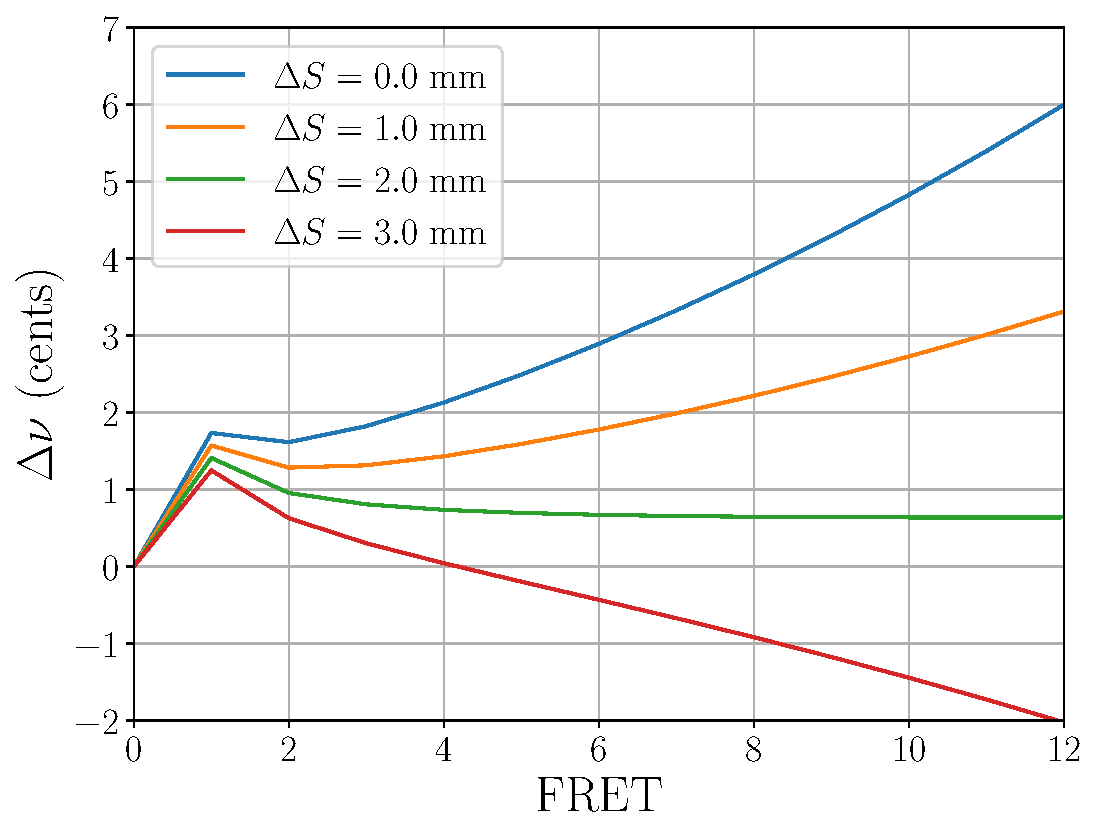
\includegraphics[width=5.0in]{figures/comp_ds}
        \caption{Frequency shifts ($\Delta N = 0$)}
        \label{fig:comp_ds}
    \end{subfigure}
    \par\vspace{0.25in}
    \begin{subfigure}[b]{0.8\textwidth}
        \centering
        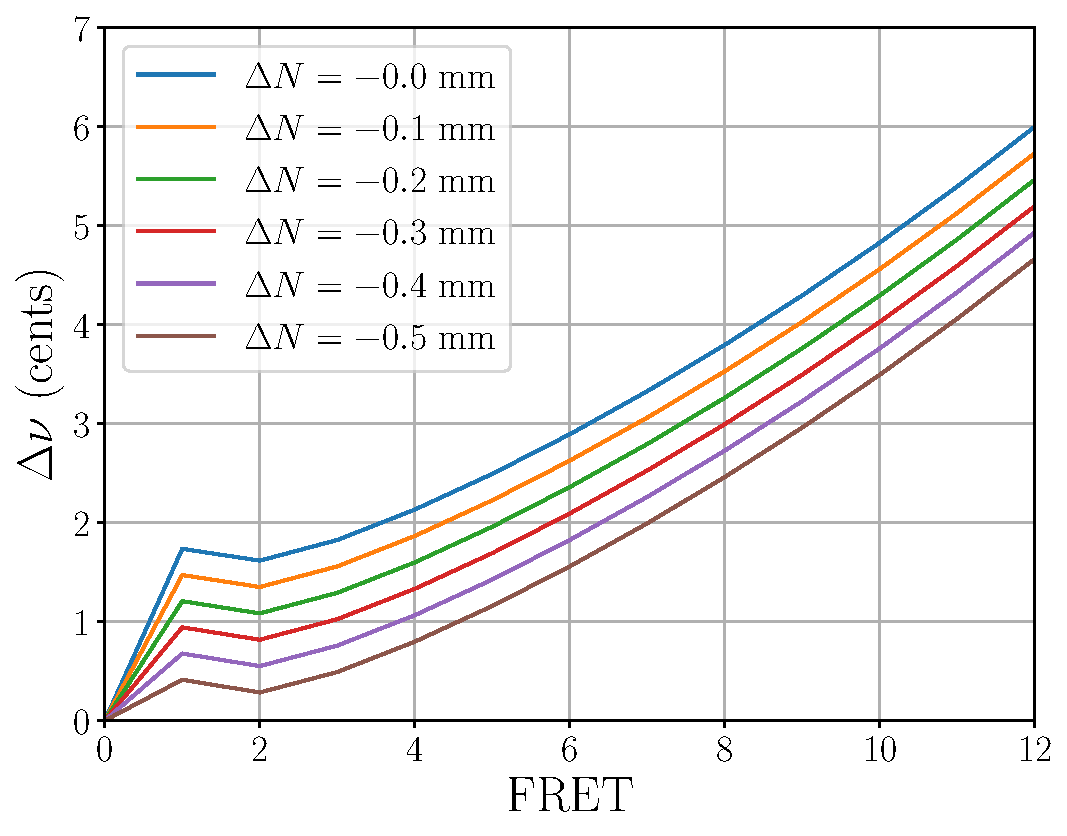
\includegraphics[width=5.0in]{figures/comp_dn}
        \caption{Frequency shifts ($\Delta S = 0$)}
        \label{fig:comp_dn}
    \end{subfigure}
    \caption{\label{fig:comp_dsdn} In (a), we plot the frequency shifts for our classical guitar for several saddle setbacks with $\Delta N = 0$. Here we use the string parameters listed in \tbl{string_specs}. In (b), we set $\Delta S = 0$ and plot the frequency shifts for several nut ``setbacks.''}
  \end{figure}
  
  % \begin{figure}
  %   \centering
  %   \begin{subfigure}[b]{0.8\textwidth}
  %       \centering
  %       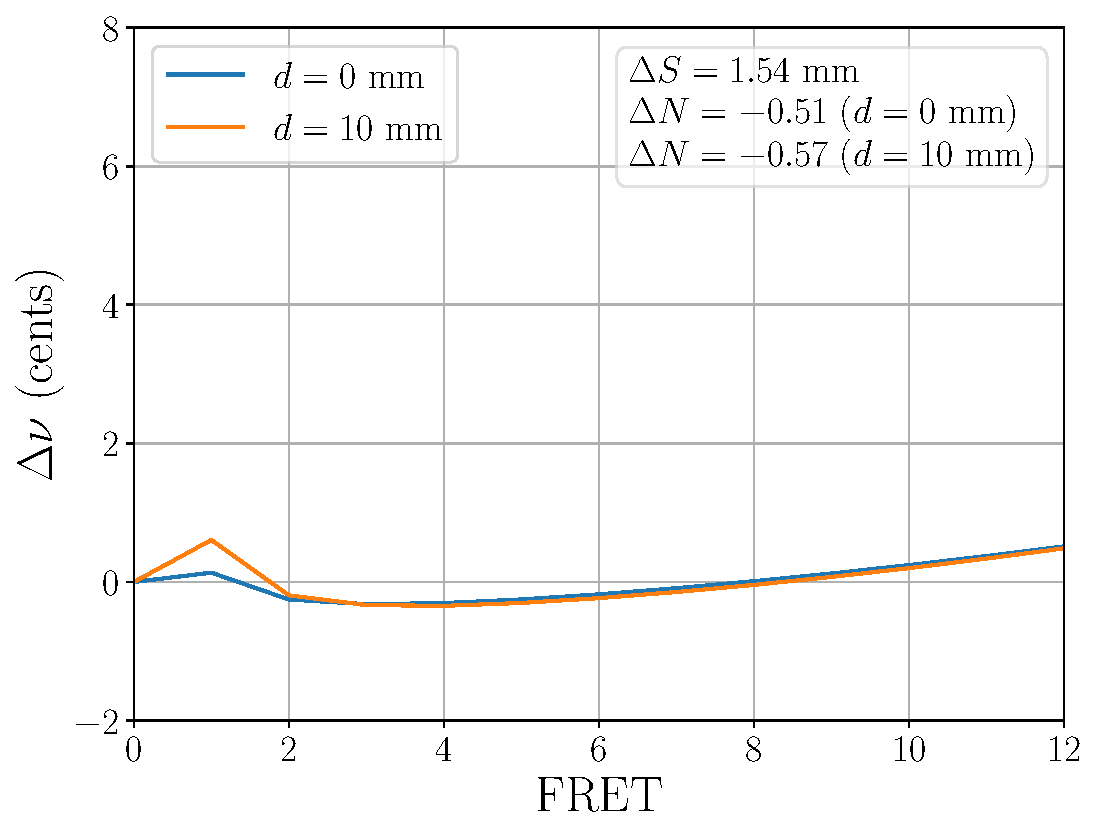
\includegraphics[width=5.0in]{figures/comp_est}
  %       \caption{Approximate compensation}
  %       \label{fig:comp_est}
  %   \end{subfigure}
  %   \par\vspace{0.25in}
  %   \begin{subfigure}[b]{0.8\textwidth}
  %       \centering
  %       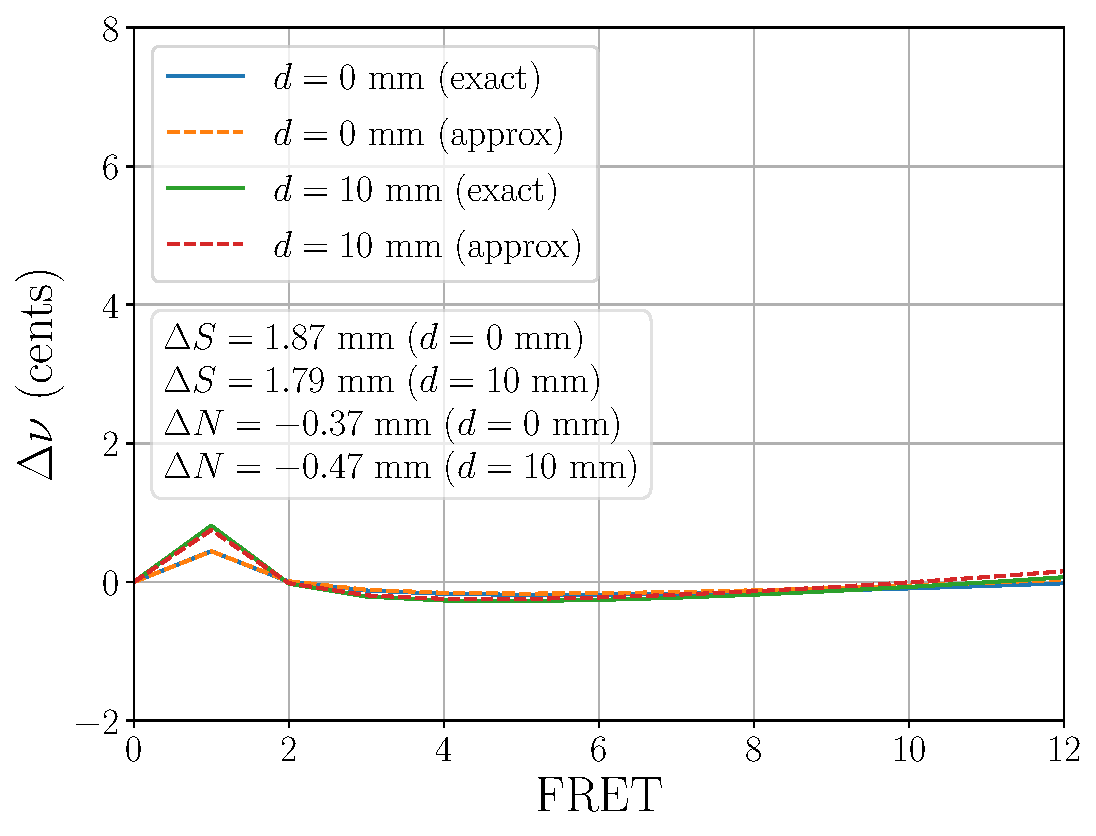
\includegraphics[width=5.0in]{figures/comp_exact}
  %       \caption{Exact compensation}
  %       \label{fig:comp_exact}
  %   \end{subfigure}
  %   \caption{\label{fig:comp_model} In (a), we plot the frequency shifts for our classical guitar with approximate setbacks computed using \eqn{comp_approx}. In (b), we compute the same setbacks }
  % \end{figure}

% \begin{figure}
%   \centering
%   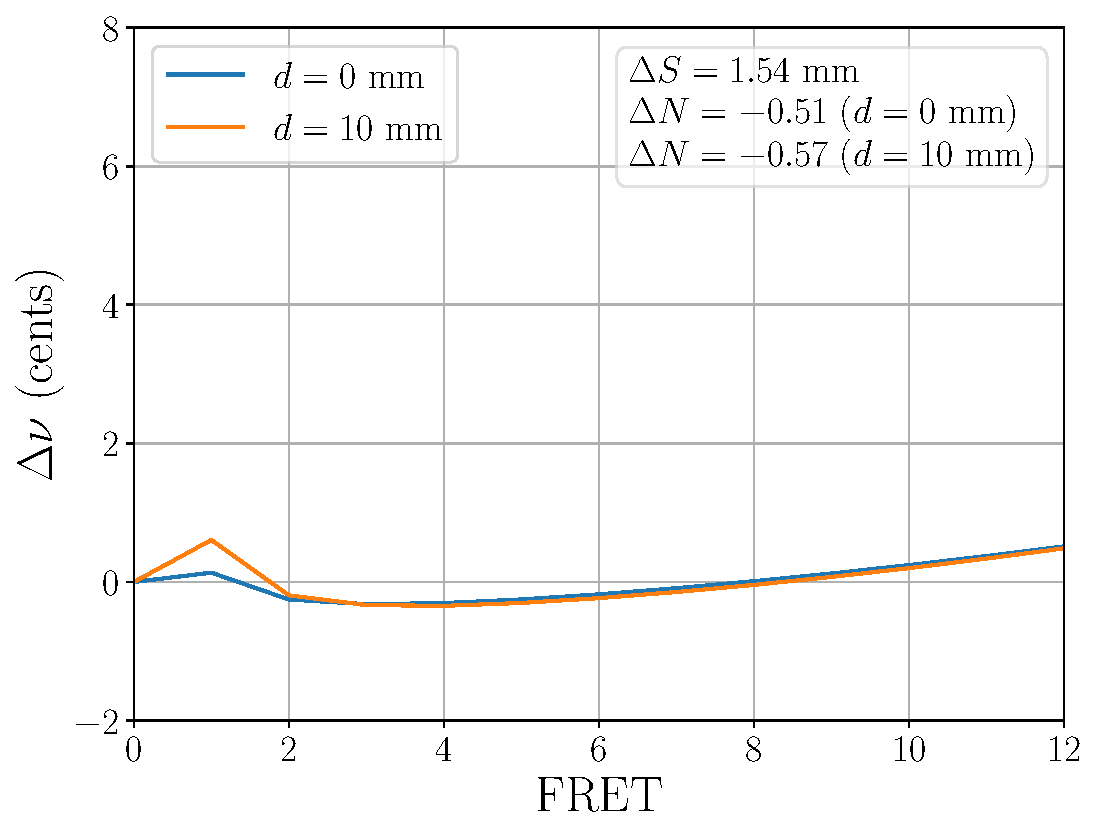
\includegraphics[width=5.0in]{figures/comp_est}
%   \caption{\label{fig:comp_est} The total frequency shift given by \eqn{error_def} for a classical guitar and string with the parameters listed in \tbl{mcg_specs} and \tbl{string_specs}, respectively.}
% \end{figure}

% Using the data and results presented in \tbl{ej45_props}, we can explore different approaches to compensating guitar strings for bending stiffness and string tension perturbations. For example, consider the guitar string shown in 

% For example, in \fig{shift_classicalguitar_ej45_factory}, using \eqn{error_def} we plot the frequency deviation (in cents) from ideal 12-TET for each string at each of the first 12 frets of an Alhambra 8P classical guitar, assuming that the open string has been perfectly tuned to the correct frequency. Recall that the Alhambra 8P is manufactured with a saddle setback of 1.5~mm, presumably to offset the effects of bending stiffness in the strings. For comparison, in \fig{shift_classicalguitar_ej45_null}, we plot the same deviations for the case where $\Delta S = 0$, which increases the error of each string at the 12$^\text{th}$ fret by 3 -- 4 cents. Recall from \sct{model} that we could crudely predict the values of the saddle and nut setbacks by inspecting \eqn{error_tot}. For example, from \tbl{ej45_props}, we estimate $\Delta S \approx B_0\, X_0 = 2.7$~mm and $\Delta N \approx -1.5$~mm for the third (G) string.


%  \begin{figure}
%   \centering
%   \begin{subfigure}[b]{0.8\textwidth}
%    \centering
%    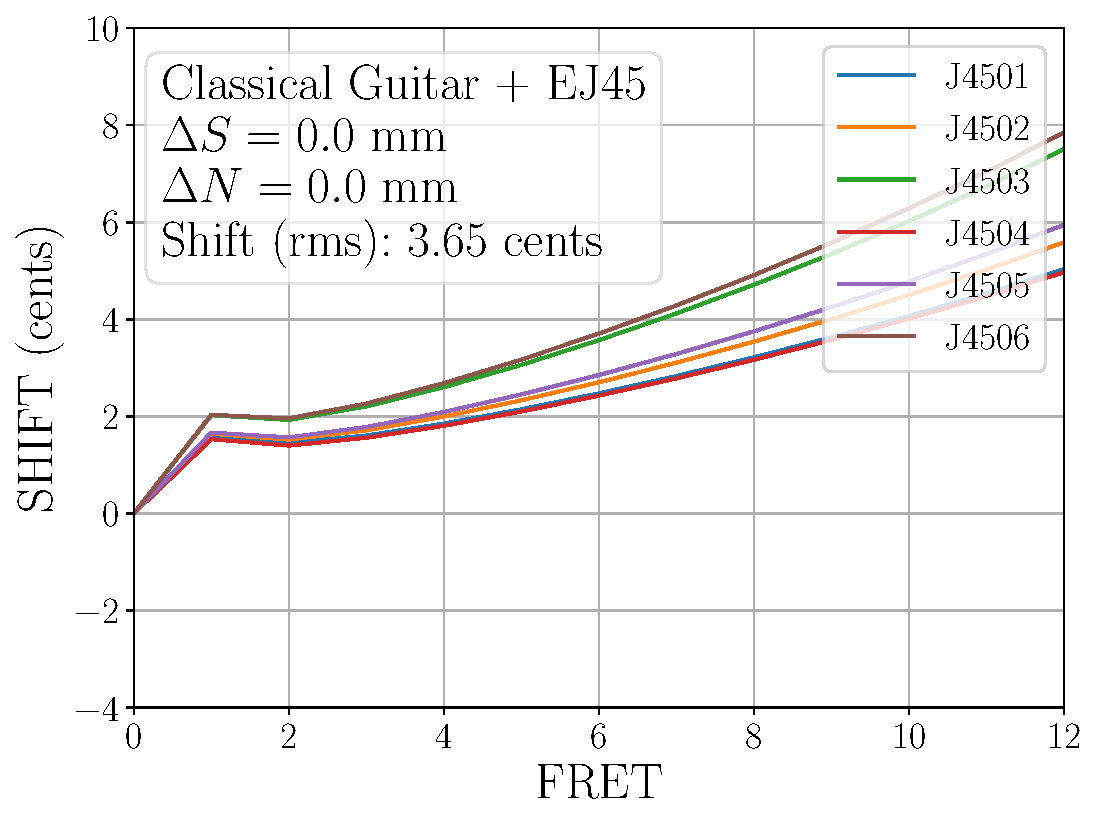
\includegraphics[width=5.0in]{figures/shift_classicalguitar_ej45_factory}
%    \caption{Factory guitar}
%    \label{fig:shift_classicalguitar_ej45_factory}
%   \end{subfigure}
%   \par\vspace{0.25in}
%   \begin{subfigure}[b]{0.8\textwidth}
%    \centering
%    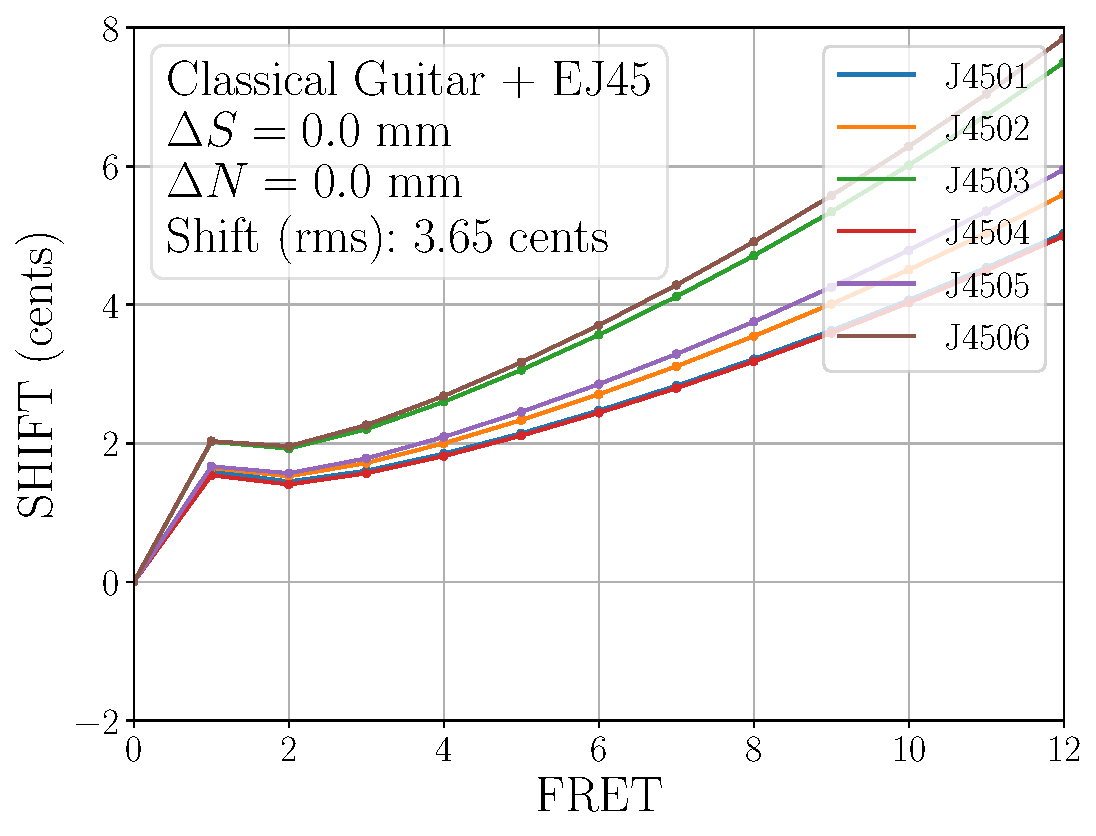
\includegraphics[width=5.0in]{figures/shift_classicalguitar_ej45_null}
%    \caption{Uncompensated}
%    \label{fig:shift_classicalguitar_ej45_null}
%   \end{subfigure}
%   \caption{\label{fig:classicalguitar_ej45} Frequency shifts (in cents) for an Alhambra 8P guitar with normal tension nylon strings (D'Addario EJ45). In (a), we show the deviations of the guitar as manufactured in the factory, completely consistent with our measurements. In (b), we show the same 12-TET errors that would arise if $\Delta S = 0$ for the same guitar.}
%  \end{figure}

As mentioned above, it is nontrivial to manufacture a guitar with different setbacks for each string~\cite{ref:byers1996cgi}, and it is unlikely that the exact values listed in \tbl{ej45_setbacks} are applicable to other string sets. We have measured the values of $R$ for five other string sets, and in \app{specs} we have reproduced the exact compensation procedure for them that we performed above for normal tension strings (with $d = 0$). Although each set exhibits variation between strings (and with respect to other sets) in individual setbacks for each string, they are similar enough that we suspect that there is the potential for great simplification in guitar design. For example, following the analysis of \app{rms}, it is possible to determine a single setback pair $\{\Delta S, \Delta N\}$ that minimizes the RMS frequency errors of an ensemble of strings over a collection of frets simply by computing the mean of the setbacks over all strings, and then using these mean values when manufacturing the guitar. If we consider five of the six string sets we have measured here --- neglecting the light tension strings because of their pathologically high values of $R$ --- we can plot the exact setback predictions shown in \fig{dsdn_mean}, and then use these results to predict the mean values. In \fig{fit_ds}, we see that the saddle setbacks are reasonably well described in terms of the string radius $\rho$ by the expression
\begin{equation}
  \Delta S = (4.4 \pm 0.2)\, \rho\, .
\end{equation}
This relationship remains true for $0 \le d \le 10$~mm. Therefore, we can either compute the mean of the saddle setbacks directly, or using the average value of the string lengths ($\overline{\rho} = 0.43 \pm 0.08$~mm). Either way, we obtain $\overline{\Delta S} = 1.8 \pm 0.4$~mm. Similarly, in \fig{hist_dn}, we show a histogram of the values of the nut setbacks, and compute the mean value $\Delta N = -0.38 \pm 0.03$~mm, which we recall is proportional to the scale length $X_0$. Note that these results are remarkably similar to the values used in \fig{shift_classicalguitar_ej45_mean}; if we plot the frequency deviations of those five string sets with these particular mean setback values, then we find that the maximum error always occurs at the twelfth fret, and it is always less than 1~cent. In the next section, we discuss a method to temper the guitar to reduce these errors further.

\begin{figure}
  \centering
  \begin{subfigure}[b]{0.8\textwidth}
   \centering
   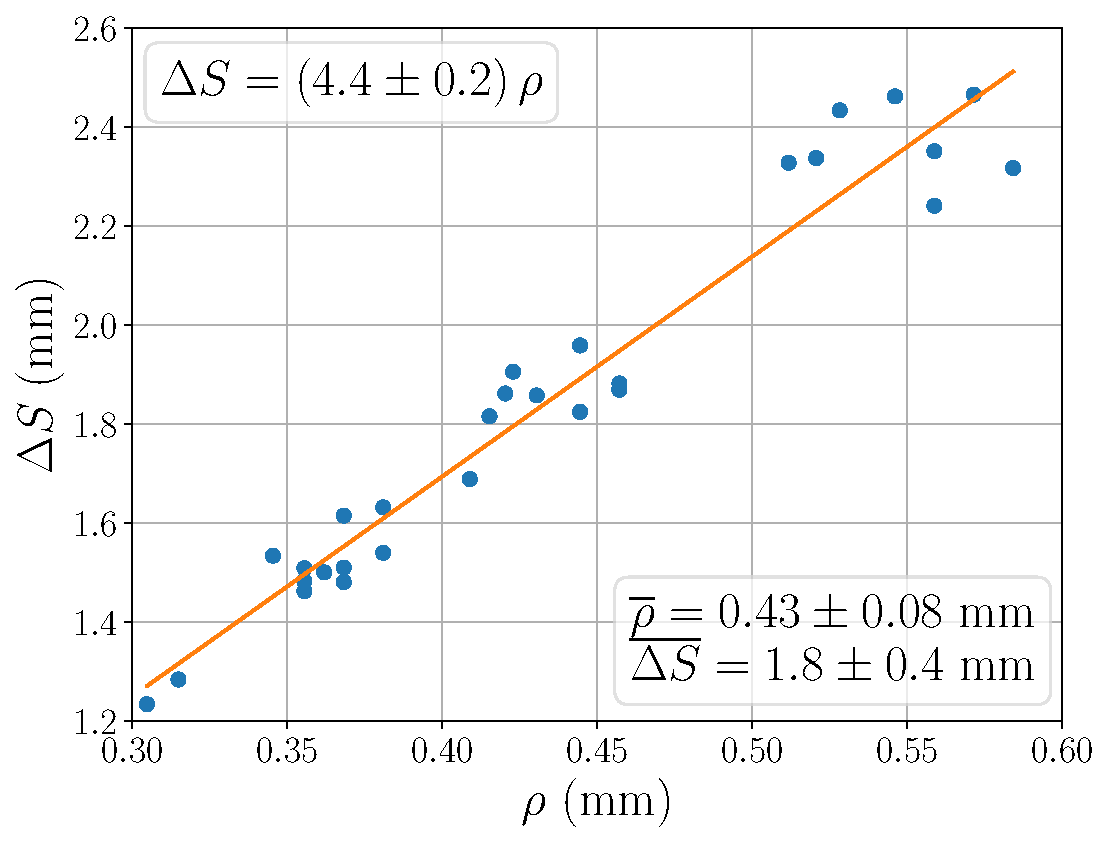
\includegraphics[width=5.0in]{figures/fit_ds}
   \caption{Five-set saddle setback data with fit}
   \label{fig:fit_ds}
  \end{subfigure}
  \par\vspace{0.25in}
  \begin{subfigure}[b]{0.8\textwidth}
   \centering
   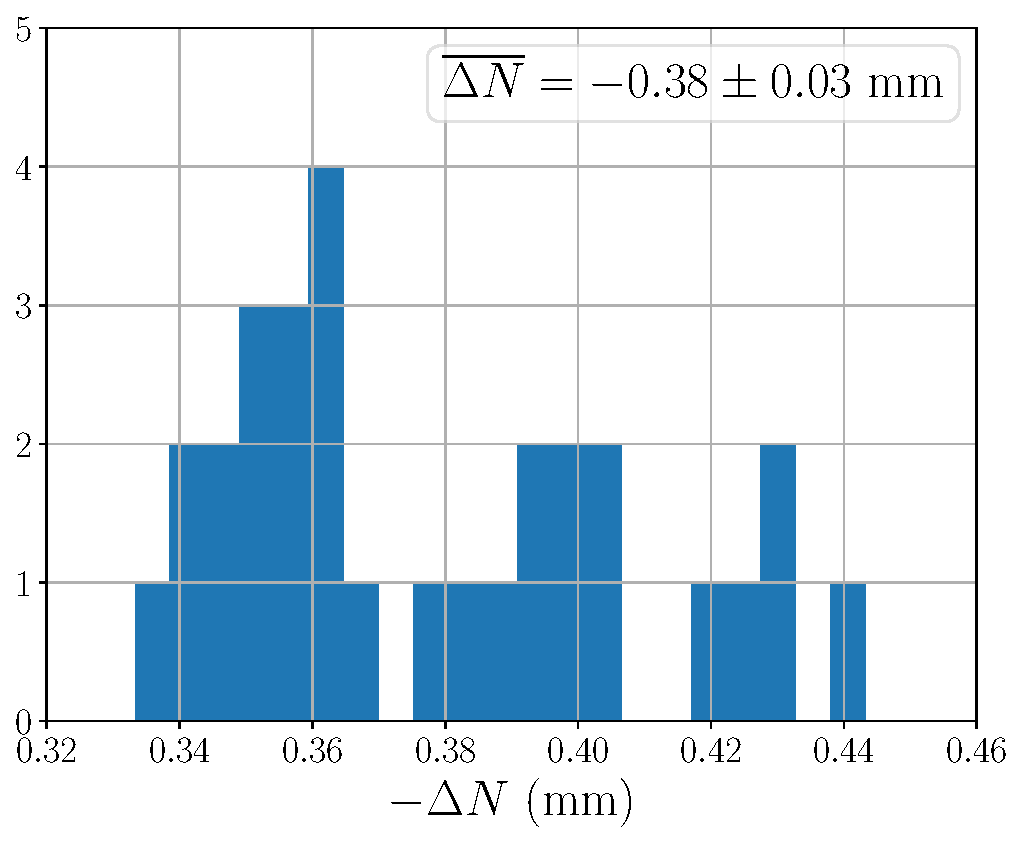
\includegraphics[width=5.0in]{figures/hist_dn}
   \caption{Five-set nut setback data with mean}
   \label{fig:hist_dn}
  \end{subfigure}
  \caption{\label{fig:dsdn_mean} Construction of mean saddle and nut setbacks over five selected string sets. In (a) we plot the saddle setback for each string as a function of the string radius, with the result of the best linear fit. In (b), we present a histogram of the nut setbacks and compute their mean.}
 \end{figure}

% Second, after paying close attention to the impact of the act of fretting on our approximations in \sct{model}, we have simply set $d = 0$ above. This is because nonzero values of $d$ have an impact on the frequency deviation of a string at the first fret, and are otherwise negligible. This tends to increase the required mean value of the nut setback, but does not require a significant change to the saddle setback. As an example, in \fig{dsdnd_ej45}, we plot the mean optimum saddle and nut setbacks for the classical guitar parameters used in \fig{shift_classicalguitar_ej45_mean} with the D'Addario Nylon Normal Tension EJ45 string set as a function of the fretting distance $d$. Paying careful attention to the $y$-axis of these plots, we see that the value of the mean saddle setback \emph{decreases} by less than 5\% as $d$ increases to 10~mm, and the magnitude of the nut setback increases by almost 30\% at the same fretting offset. This behavior is essentially the same for all string sets considered in this work, and can be used by the luthier to determine the optimum setback values for their designs. Note that --- when the RMS approach is used to compute the mean setbacks --- the difference $\Delta S - \Delta N$ (the sum of the saddle setback and the magnitude of the nut setback) is virtually independent of $d$, as shown in \fig{dsnd_ej45}. We see here that the distance between the saddle and the nut \emph{does not depend on} $d$; as $d$ increases, the saddle and the nut move together toward the guitar bridge at lower $x$ values. Therefore, for values of $b$ and $c$ that are within 50\% of those listed in \tbl{mcg_specs}, we can fit the change of $\Delta N$ to a polynomial in $d/X_0$, and find
% \begin{align} \label{eqn:comp_d_poly}
%   \Delta N(d) &\approx \Delta N(0) \left[ 1 + 13\, (d/X_0) + 280\, (d/X_0)^2 \right]\, , \nd \\
%   \Delta S(d) &\approx \Delta S(0) + \Delta N(0) \left[13\, (d/X_0) + 280\, (d/X_0)^2 \right]\, .
% \end{align}
% As $d$ increases, the magnitude of the negative nut setback increases, and the saddle setback decreases because $\Delta N < 0$. Updating the guitar string illustrated in \fig{comp_est}, and using both \eqn{rms_sol_quad} with \emph{no} approximations (``exact'') and \eqn{rms_sol_comp} with \eqn{comp_d_poly} (``approx''), we find the setbacks and show the corresponding frequency deviations in \fig{comp_exact}. The setback values computed using these two methods are virtually identical.

% \begin{figure}
%   \centering
%   \begin{subfigure}[b]{0.8\textwidth}
%       \centering
%       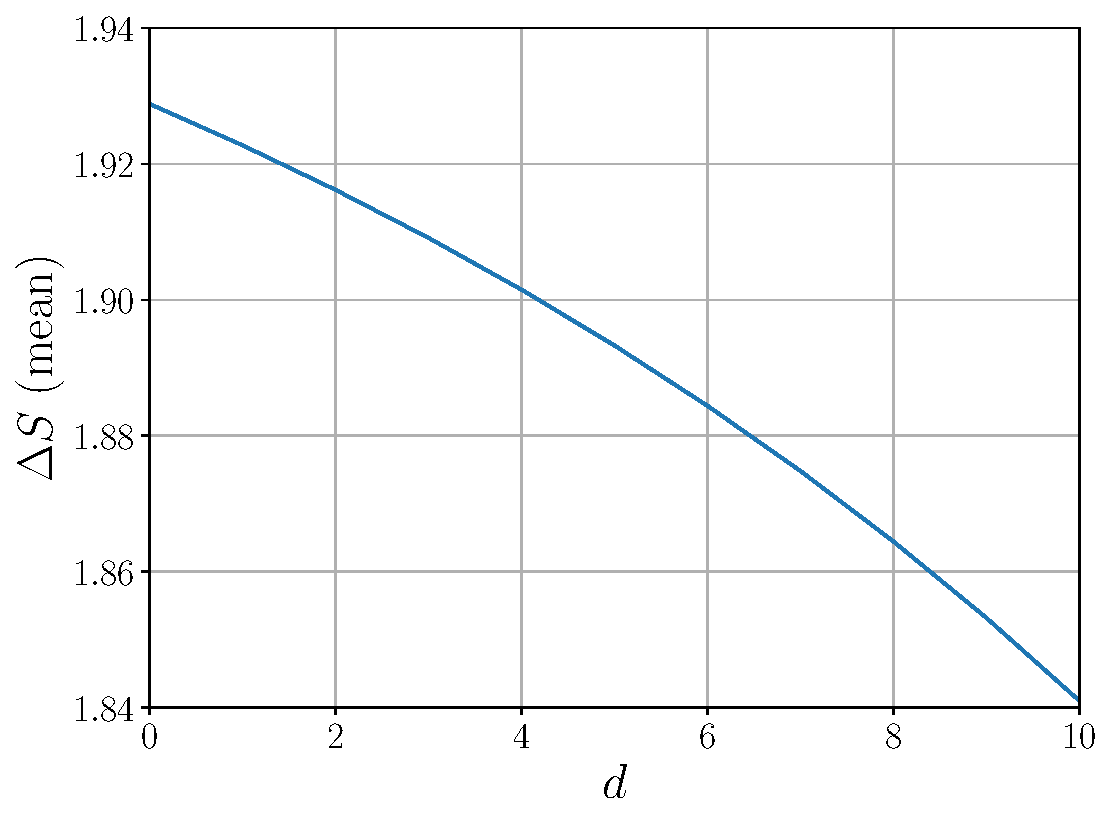
\includegraphics[width=5.0in]{figures/dsd_ej45}
%       \caption{Mean saddle setback}
%       \label{fig:dsd_ej45}
%   \end{subfigure}
%   \par\vspace{0.25in}
%   \begin{subfigure}[b]{0.8\textwidth}
%       \centering
%       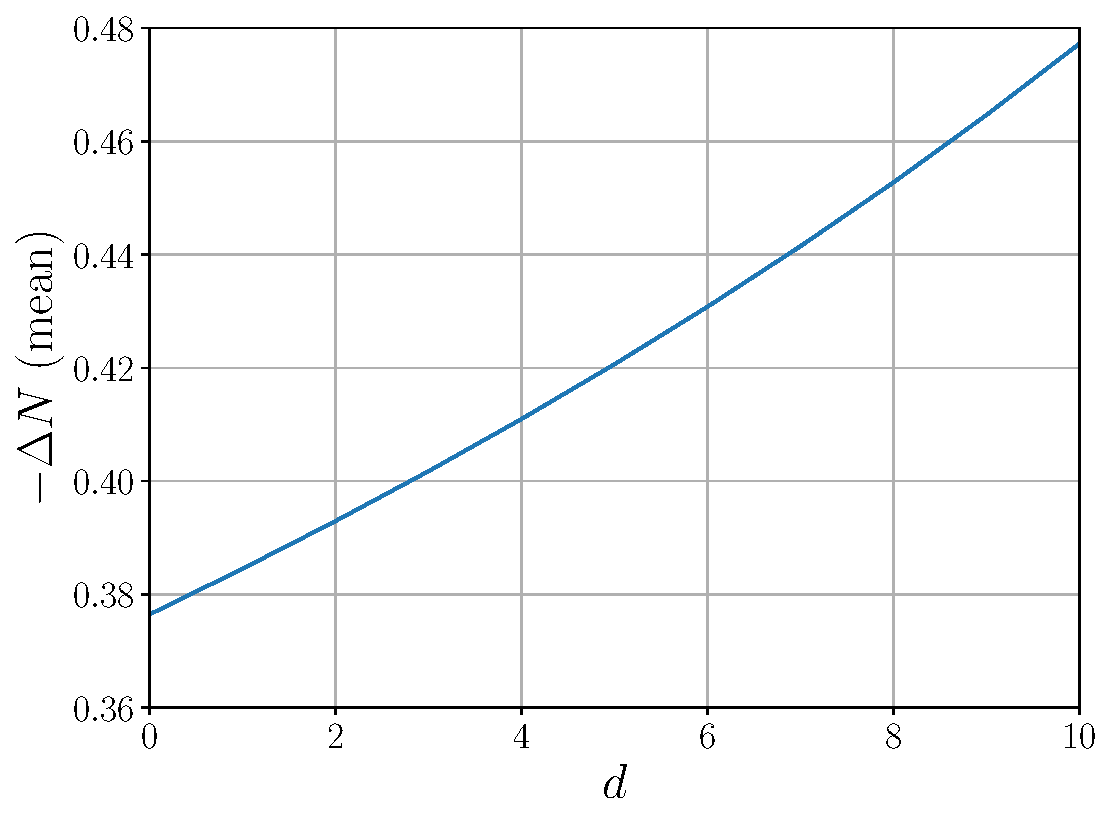
\includegraphics[width=5.0in]{figures/dnd_ej45}
%       \caption{Mean nut setback}
%       \label{fig:dnd_ej45}
%   \end{subfigure}
%   \caption{\label{fig:dsdnd_ej45} The mean optimum saddle and nut setbacks for the D'Addario Nylon Normal Tension EJ45 string set as a function of the fretting distance $d$.}
% \end{figure}

% \begin{figure}
%   \centering
%   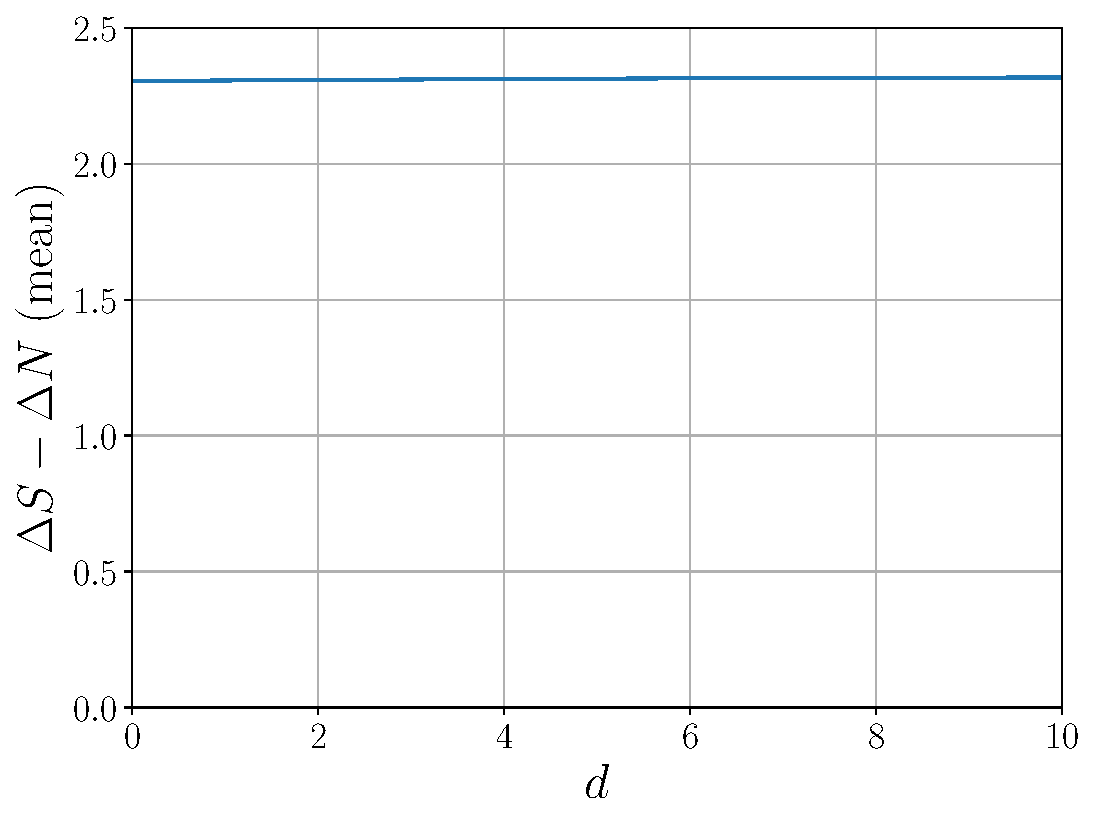
\includegraphics[width=5.0in]{figures/dsnd_ej45}
%   \caption{\label{fig:dsnd_ej45} The mean value of $\Delta S - \Delta N$ for the D'Addario Nylon Normal Tension EJ45 string set as a function of the fretting distance $d$.}
% \end{figure}

% \begin{figure}
%   \centering
%   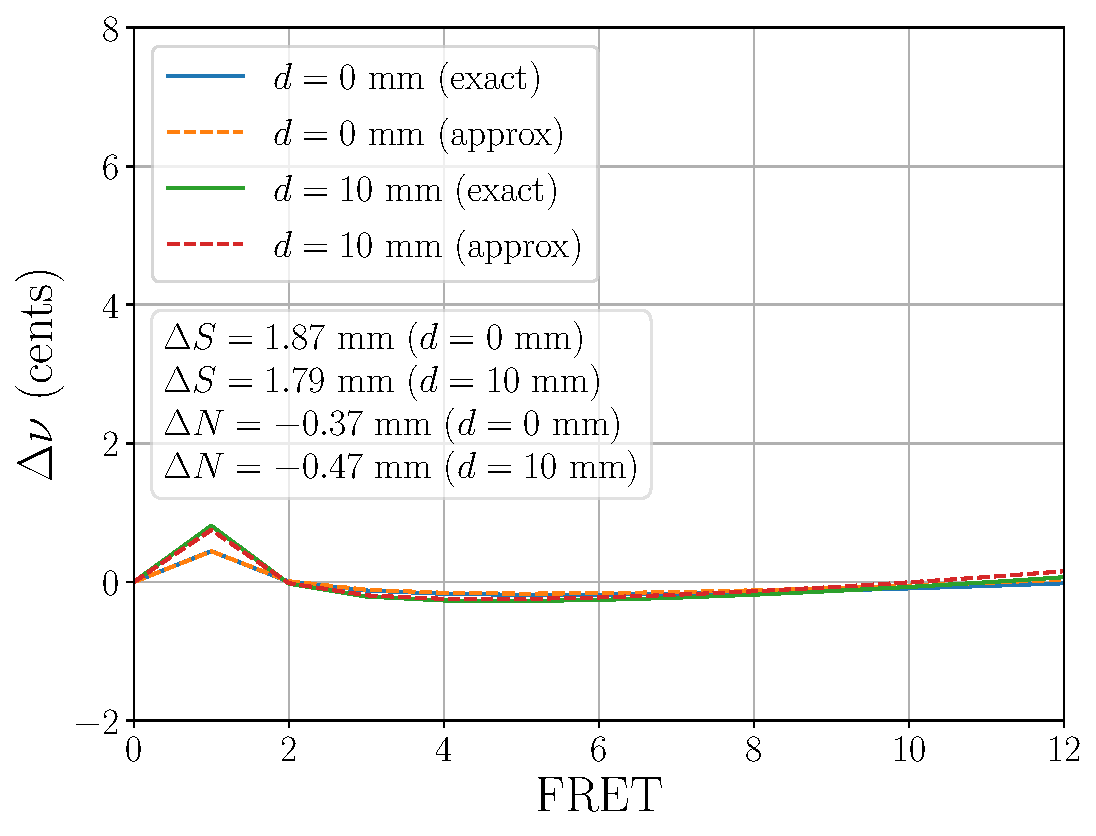
\includegraphics[width=5.0in]{figures/comp_exact}
%   \caption{\label{fig:comp_exact} The total frequency shift given by \eqn{error_def} for a classical guitar with setbacks computed using both \eqn{rms_sol_quad} with \emph{no} approximations (``exact'') and \eqn{rms_sol_comp} with \eqn{comp_d_poly} (``approx'').}
% \end{figure}
